% !TEX root = flow_head.tex


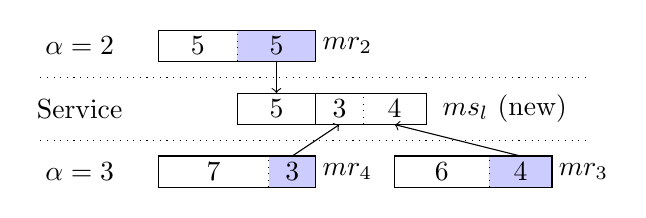
\begin{tikzpicture}
\fill[blue!20!] (10mm,0) rectangle (20mm,4mm);
\draw (0,0) rectangle (20mm,4mm) (24mm,2mm) node{$mr_2$};
\draw (5mm,2mm) node{5} (15mm,2mm) node{5} (-1cm,2mm) node{$\alpha=2$} (12mm,2mm);
\draw[dotted] (10mm,0) -- (10mm,4mm);

\draw[->] (15mm,0) edge (15mm,-4mm) (17mm,-12mm) edge (23mm,-8mm) (46mm,-12mm) edge (30mm,-8mm);
% \draw[->,xshift=30mm](41mm,-12mm) edge (20mm,-8mm);

\draw[dotted,yshift=-2mm] (-1.5cm,0) -- (5.5cm,0);

\draw[yshift=-8mm,xshift=10mm] (0,0) rectangle (24mm,4mm) (34mm,2mm) node{$ms_l$ (new)};
\draw[yshift=-8mm,xshift=10mm] (10mm,0) -- (10mm,4mm);
\draw[yshift=-8mm,dotted,xshift=10mm] (16mm,0) -- (16mm,4mm);
\draw[yshift=-8mm,xshift=10mm] (5mm,2mm) node{5} (13mm,2mm) node{3} (20mm,2mm) node{4} (-2cm,2mm) node{Service};

\draw[dotted,yshift=-10mm] (-1.5cm,0) -- (5.5cm,0);

\fill[blue!20!,yshift=-16mm] (14mm,0) rectangle (20mm,4mm);
\fill[blue!20!,yshift=-16mm,xshift=30mm](20mm,4mm) rectangle +(-8mm,-4mm);
\draw[yshift=-16mm] (0,0) rectangle (20mm,4mm) (24mm,2mm) node{$mr_4$};
\draw[yshift=-16mm,xshift=30mm] (0,0) rectangle (20mm,4mm) (24mm,2mm) node{$mr_3$};
\draw[yshift=-16mm,dotted] (14mm,0) -- +(0,4mm) ;
\draw[yshift=-16mm,dotted,xshift=30mm] (12mm,0) -- +(0,4mm);
\draw[yshift=-16mm] (7mm,2mm) node{7} (17mm,2mm) node{3} (-1cm,2mm) node{$\alpha=3$};
\draw[yshift=-16mm,xshift=30mm] (6mm,2mm) node{6} (16mm,2mm) node{4};
\end{tikzpicture}
